\setbeamertemplate{caption}{\raggedright\insertcaption\par}
\captionsetup[figure]{labelformat=empty}% redefines the caption setup of the figures environment in the beamer class.

\section{Motivation}

\frame{\frametitle{Fatigue damage}

\uncover<1->{
		\twocol{	\begin{itemize}
				\item Fluctuating loads
			\end{itemize}
			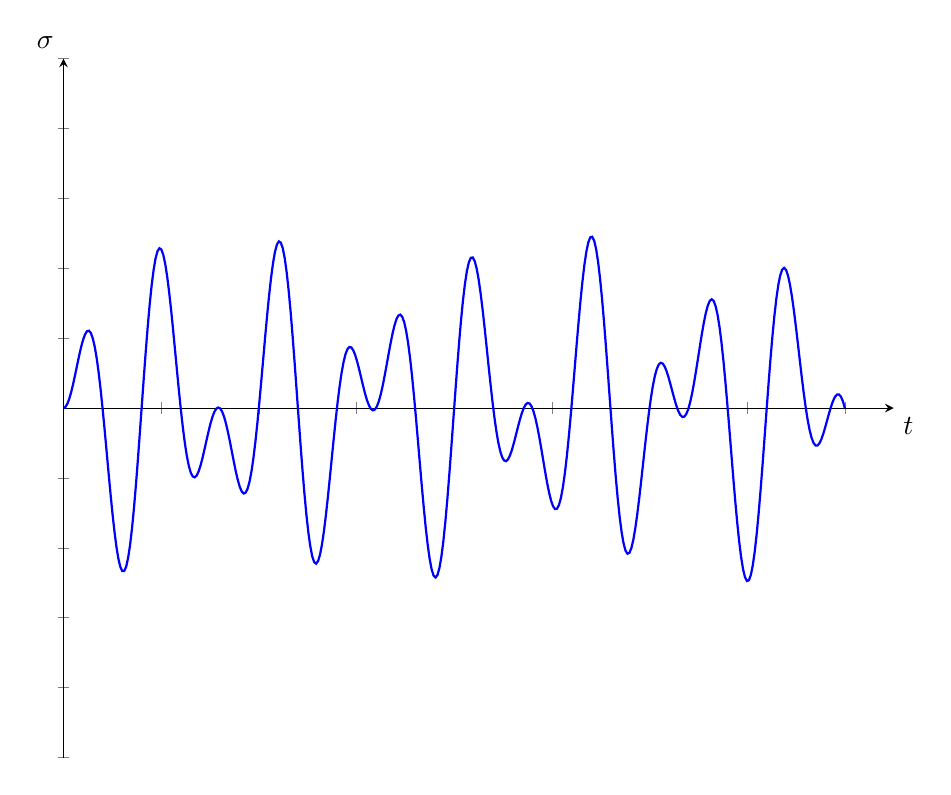
\begin{tikzpicture}[scale=1]
			\begin{axis}[axis x line=center, axis y line=center,
			xticklabels={},yticklabels={},xlabel style={below right},
			ylabel style={above left},ymin=-1,ymax=1,xmin=0,xmax=8.5,
			width=\textwidth,xlabel=$t$,ylabel=$\sigma$]
			\addplot [color=blue,thick,mark=none,domain=0:8,samples=400]{sin(2*\x r)*0.5*sin(pi / 2 * 5 * \x r)} ;
			\end{axis}
			\end{tikzpicture}
		}{
			\centering
			\uncover<2->{\hfil
				\begin{itemize}
					\item Material degradation\\[0.6cm]
				\end{itemize}

					\only<2>{\includegraphics[width=0.9\textwidth]{/home/alameddin/src/tex/templates/figures/windturbine.jpg}\\[-0.3cm]}

					\only<3->{\includegraphics[width=0.9\textwidth]{/home/alameddin/src/tex/templates/figures/bridge.jpg}\\[-0.3cm]}
					\uncover<2-3>{\vspace*{0.1cm} {\tiny Image by alegri / 4freephotos.com}}

				}

				}
			}
			{

			}
	}



\frame{\frametitle{Fatigue damage}

		\twocol{	\begin{itemize}
				\item Fluctuating loads
			\end{itemize}
			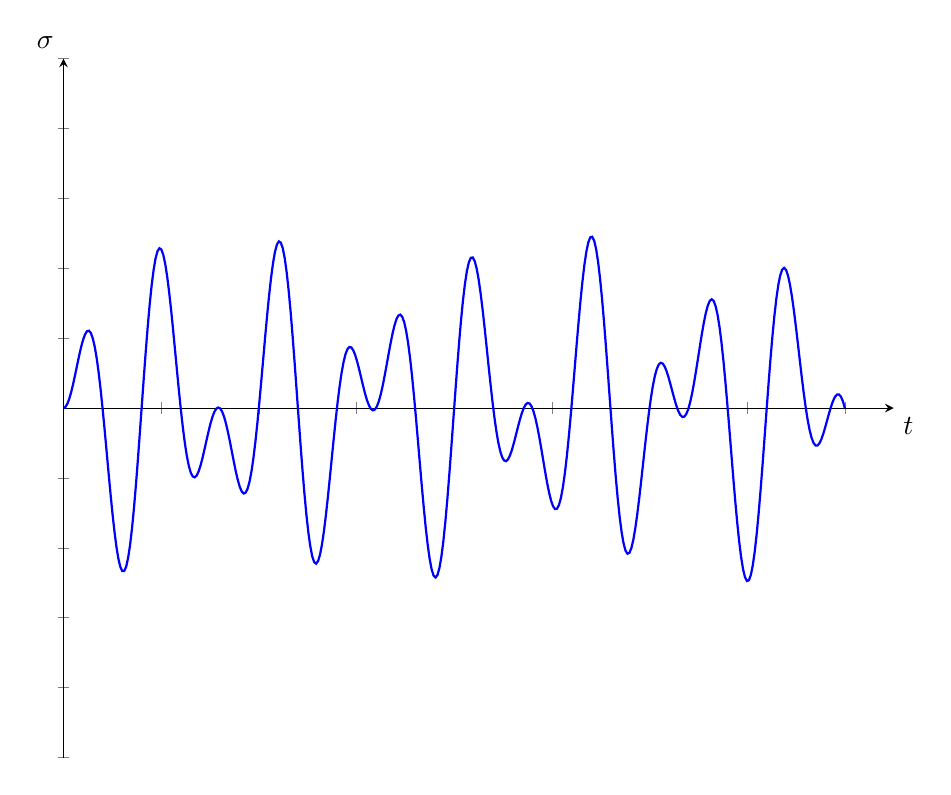
\begin{tikzpicture}[scale=1]
			\begin{axis}[axis x line=center, axis y line=center,
			xticklabels={},yticklabels={},xlabel style={below right},
			ylabel style={above left},ymin=-1,ymax=1,xmin=0,xmax=8.5,
			width=\textwidth,xlabel=$t$,ylabel=$\sigma$]
			\addplot [color=blue,thick,mark=none,domain=0:8,samples=400]{sin(2*\x r)*0.5*sin(pi / 2 * 5 * \x r)} ;
			\end{axis}
			\end{tikzpicture}
		}{
			\centering
			\uncover<1->{\hfil
				\uncover<1->{	\begin{itemize}
						{\item Virtual experiments\\[0.5cm]}
						{\item Continuum damage model\\[0.5cm]}
						{\item Millions of cycles\\[0.5cm]}
						{\item Macro crack initiation \\[0.5cm]}
						{\item Computationally expensive\\[0.5cm]}
					\end{itemize}}
				}
			}
			{
				\uncover<2>{
					\begin{block}{ \centering Model order reduction (MOR) techniques}
					\end{block}

				}
			}
		}


\section{LATIN framework}

\frame{\frametitle{State of the art}
		\begin{itemize}
			{\item \small An approach to include damage in a LATIN-PGD framework \dSmiley \\[0.5cm]}
			{\item \small Two-time scale approach to tackle large number of cycles \dSmiley \\[1cm]}
			{\item \small Limited to specific damage models \frownie{}\\[0.5cm]}
			{\item \small Inefficient for high damage values \frownie{} \\[0.5cm]}
			{\item \small Not easy to include variable amplitude loads \frownie{}\\
			\quad	without the two-time scale:\\ \qquad	no time savings and many modes are generated\\[0.5cm]}
		\end{itemize}
}

\frame{\frametitle{Goals}
	\begin{itemize}
		{\item \small Generalised formulation for different nonlinear material models\\[0.5cm]}
		\quad $\bullet$ {\small Tackle high damage values\\[0.5cm]}
		\quad $\bullet$ {\small Efficient in comparison with classical damage approaches\\[0.5cm]}
		{\item \small Variable amplitude loading \\[0.5cm]}
		{\item \small Decouple the problem dimensionality from the high fidelity one\\[0.5cm]}
	\end{itemize}
}

\frame{\frametitle{Mechanical problem}
	\begin{block}{ \centering Equilibrium equation}
	\end{block}
\vspace{-0.5cm}
\begin{minipage}[t]{0.4\textwidth}
	\begin{itemize}
		{\item Static admissibility }
		\vspace{-0.5cm}
		\begin{align*}
		\div{\fsigma}+\fb&=\fzero \text{ in } \mathrm{\Omega}\\
 		u&=\bar{u} \text{ in } \mathrm{\partial\Omega}_{\mathrm{D}}
		\end{align*}
	\end{itemize}
\end{minipage}\hfil\begin{minipage}[t]{0.5\textwidth}
	\begin{itemize}
		{\item Kinematic admissibility}
		$\feps = \grads{u}$
	\end{itemize}
\end{minipage}

	\begin{block}{ \centering Nonlinear material model}
	\end{block}
\vspace{-0.5cm}
\begin{minipage}[t]{0.4\textwidth}
	\begin{itemize}
		{\item State equations}
		\vspace{-0.3cm}
		\begin{equation*}
		\begin{split}
		\fsigma &=\pd{\psi}{\fepse} \\
		\fbeta &= \pd{\psi}{\falpha}\\
		Y &=-\pd{\psi}{D}
		\end{split}
		\end{equation*}
	\end{itemize}
\end{minipage}\hfil\begin{minipage}[t]{0.5\textwidth}
	\begin{itemize}
		{\item Evolution equations}
				\vspace{-0.3cm}
		\small
		\begin{equation*}
		\begin{split}
		{\dot{\epst}}^{\rm p} &= \pd{\phi^{\rm p}}{\sig}\\
		{\dot\alpha} &=- \pd{\phi^{\rm p}}{\beta} \\
		{\dot{D}} &= \pd{\phid}{D}
		\end{split}
		\end{equation*}
	\end{itemize}
\end{minipage}

}

\frame{\frametitle{Solution algorithm}
	\begin{itemize}
		{\item Many LATIN algorithms since 1985 }
		{\item A combination with some modifications}
			\begin{itemize}
				{\item First stage (local)}	\\
					$\bullet$ Solve all local equations (possibly in parallel),\\ \quad given initial conditions
				{\item Second stage (global)}\\
					$\bullet$ Solve all global equations
				{\item Data flow between these stages}
				\vspace{-0.3cm}
				\begin{equation*}
				\begin{split}
				(\stepj[]{\fsigma}-\stepi[]{\fsigma}) \; +  {\ffH^+} \ \; (\stepj[]{\feps}-\stepi[]{\feps}) \ \; &=\fzero\\
				(\stepk[ ]{\fsigma}-\stepj[ ]{\fsigma}) -{\ffH^-}(\stepk[]{\feps}-\stepj[]{\feps})&= \fzero
				\end{split}
				\end{equation*}
				{\item Iterate until convergence \\[0.5cm]}
			\end{itemize}
	\end{itemize}
}

\frame{\frametitle{The global stage}
		\begin{itemize}
			\item  The solution is approximated by a finite sum of separated functions (low-rank approximation)
			\begin{equation*}
			{u}(x,t)=\ds \sum_{i=1}^{N} \lambda_i(t) \ \bar{u}_i(x)
			\end{equation*}
			\item  Static admissibility
			\begin{equation*}
			\small
			\begin{split}
			\left( \intT  \ \lambda^2 \d t \right) \intS \grad{v}^\ast \ffC \grad{v} \ \d \Omega = - \intS \grad{v}^\ast \left( \intT \lambda \ \hf \d t \right)  \d \Omega\\
			\intT \lambda^\ast \left( \intS  \grad{v} \ \ffC \ \grad{v} \d \Omega \right) \lambda \ \d t = - \intT \lambda^\ast \left( \intS  \grad{v} \ \hf \d \Omega \right)  \d t
			\end{split}
			\end{equation*}
	\end{itemize}
%		\mediabutton[jsaction={anim.myAnim.playFwd();}]{\fbox{\strut Play}}
%		\mediabutton[jsaction={anim.myAnim.pause();}]{\fbox{\strut Pause}}
	%		 \includegraphics[width=0.4\linewidth]{./img/lating-0.png}
\begin{center}
%	\includegraphics[width=0.7\textwidth]{./fig_new/inter.png}\\[-0.3cm]
\end{center}
}

\frame{\frametitle{Algorithmic point of view}
	\begin{itemize}
		\item One cycle
		\begin{equation*}
		\small
		\begin{split}
			\gamma \ \mK \ \vec{v} &= \vec{F} \qquad (n \times n)\\
			\mA \ \vlambda &= \vb  \qquad (n_t \times n_t)
		\end{split}
		\end{equation*}
		\item Multiple cycles with variable load amplitudes\\
			$\bullet$ The initial stiffness\\
			\uncover<2>{\qquad compute only once\\}
			$\bullet$ The elastic solution\\
			\uncover<2>{\qquad compute only once\\}
			$\bullet$ An initial guess\\
			\uncover<2>{\qquad from the previous cycle\\}			
	\end{itemize}
}

\frame{\frametitle{Numerical results}
	\begin{itemize}
		\item Validation
		\begin{figure}[htbp!]
			\centering
			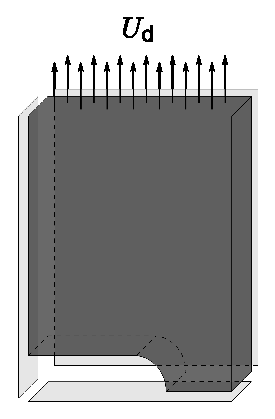
\includegraphics[scale=0.7,clip]{/home/alameddin/src/tex/templates/figures/3d_plate_1_8.eps}
		\end{figure}
	\end{itemize}
	 \begin{center}
			A plate with a central groove subjected to cyclic loading\\ (Cr-Mo steel at $580^\circ \rm C$)
	\end{center}
}

\frame{\frametitle{Numerical results}

\twocol{\begin{figure}
		\includegraphics[width=0.9\linewidth]{/home/alameddin/src/tex/templates/figures/euromech/neon_damage.png}\\
		{Newton-Raphson}
\end{figure}}{\begin{figure}
\includegraphics[width=0.9\linewidth]{/home/alameddin/src/tex/templates/figures/euromech/latin_damage.png}\\
\centering{LATIN-PGD}
\end{figure}}{\centering
Damage contour after at the last time step\\
}

}

\frame{\frametitle{Numerical results}

\twocol{\begin{figure}
		\includegraphics[width=0.9\linewidth]{/home/alameddin/src/tex/templates/figures/euromech/neon_stress.png}\\
		{Newton-Raphson}
\end{figure}}{\begin{figure}
\includegraphics[width=0.9\linewidth]{/home/alameddin/src/tex/templates/figures/euromech/latin_stress.png}\\
{LATIN-PGD}
\end{figure}}{\centering
Residual stress distribution after removing the load
}
}

\frame{\frametitle{Variable amplitude}
	\twocol{\begin{figure}
			\centering
				\vspace{1cm}
			\includegraphics[width=0.9\textwidth]{/home/alameddin/src/tex/templates/tex_figures/variable_load_12cycles.pdf}
	\end{figure}}{\begin{figure}
	\centering
	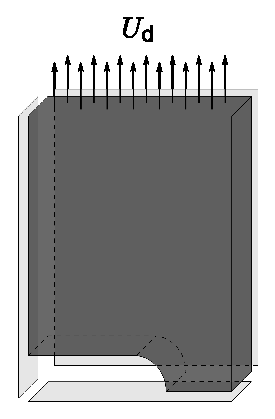
\includegraphics[scale=0.7,clip]{/home/alameddin/src/tex/templates/figures/3d_plate_1_8.eps}
	\end{figure}}{ }
}
\frame{\frametitle{Variable amplitude}
	\twocol{\begin{figure}
		\includegraphics[width=0.9\linewidth]{/home/alameddin/src/tex/templates/tex_figures/damage_12cycles.pdf}
%		\caption{Damage w.r.t. number of cycles}
		\label{fig_damage_evolution12cycles}
	\end{figure}}{\begin{figure}
		\includegraphics[width=0.9\linewidth]{/home/alameddin/src/tex/templates/tex_figures/number_pgdmodes_12cycles.pdf}
%		\caption{Number of PGD modes in each cycle}
		\label{fig_pgdmodes12cycles}
	\end{figure}}{}
}

\frame{\frametitle{Variable amplitude}
\twocol{\begin{figure}
	\includegraphics[width=0.9\linewidth]{/home/alameddin/src/tex/templates/figures/euromech/damage_12cycles.png}
	\caption{Damage distribution}
\end{figure}}{\begin{figure}
	\includegraphics[width=0.9\linewidth]{/home/alameddin/src/tex/templates/figures/euromech/residual_vonmises_12cycles.png}
	\caption{Von Mises stress distribution}
\end{figure}}{}
}

\frame{\frametitle{Variable amplitude}
\twocol{\begin{figure}
	\includegraphics[width=0.82\linewidth]{/home/alameddin/src/tex/templates/tex_figures/iterations_12cycles.pdf}
%	\caption{Number of iteration}
\end{figure}}{\begin{figure}
	\includegraphics[width=1\linewidth]{/home/alameddin/src/tex/templates/tex_figures/error_12cycles.pdf}
%	\caption{Error indicator}
	\label{fig_err_12cycles}
\end{figure}}{}
}

\frame{\frametitle{Overloads}
	\vspace{0.8cm}
	{\begin{figure}
			\centering
			\includegraphics[width=0.6\linewidth]{/home/alameddin/src/tex/templates/tex_figures/overload.pdf}
	\end{figure}}
}

\frame{\frametitle{Random amplitudes}
	\vspace{0.8cm}
	\only<1>{\begin{figure}
			\centering
			\includegraphics[width=0.6\linewidth]{/home/alameddin/src/tex/templates/tex_figures/randomload0.pdf}
	\end{figure}}
	\only<2>{\begin{figure}
			\centering
			\includegraphics[width=0.6\linewidth]{/home/alameddin/src/tex/templates/tex_figures/randomload1.pdf}
	\end{figure}}
	\only<3>{\begin{figure}
			\centering
			\includegraphics[width=0.6\linewidth]{/home/alameddin/src/tex/templates/tex_figures/randomload2.pdf}
	\end{figure}}
	\only<4>{\begin{figure}
			\centering
			\includegraphics[width=0.6\linewidth]{/home/alameddin/src/tex/templates/tex_figures/randomload3.pdf}
	\end{figure}}
	\only<5>{\begin{figure}
			\centering
			\includegraphics[width=0.6\linewidth]{/home/alameddin/src/tex/templates/tex_figures/randomload4.pdf}
	\end{figure}}
%	\only<6>{\begin{figure}
%			\centering
%			\includegraphics[width=0.6\linewidth]{/home/alameddin/src/tex/templates/tex_figures/randomload5.pdf}
%	\end{figure}}	
	\uncover<6-7>{\begin{figure}
			\centering
			\includegraphics[width=0.6\linewidth]{/home/alameddin/src/tex/templates/tex_figures/randomload_damage.pdf}
	\end{figure}}
	\uncover<7>{\begin{block}{ \centering Speed-up factor $\sim$ 50}
	\end{block}}

}



\frame{\frametitle{Conclusion and future research}
	\begin{minipage}[t]{0.5\textwidth}
		\begin{itemize}
			\item Efficient cycle by cycle simulation
			\item Works for LCF and HCF
		\end{itemize}
	\end{minipage}\begin{minipage}[t]{0.5\textwidth}
		\begin{itemize}
			\item POD approach			
			\item Time adaptivity
			\item Modes selection
			\item Faster orthogonalisation
			\item Hyper-reduction
		\end{itemize}
	\end{minipage}
\vfill

	\uncover<2>{\begin{block}{ \centering Thank you for your attention}
	\end{block}}
}


% 12 cycles
%main(linspace(33,66,12)*1e-4)

% random load 
%r = ones(1,100) * 42e-4;
% r(4:6) = 52e-4;
%r(49:51) = 52e-4;
% r(94:96) = 52e-4;